\textbf{Please explain all your filled-in codes with a snapshot of those lines of code. List formulas you have used for that part of code.}\\
The code block is used to simulate the motion model of the UAV in the SLAM system by making sure that it updates each particle's position and orientation accounting for noise to ensure that the system takes into account uncertainties in movement. The task requires applying rotation and translation to the particles through the inclusion of noise in the uncertainty calculation within SLAM. Need to update the rotation noise (angle $\theta$) of each particle using some random noise, which includes both additive and proportional noise components (constant noise and proportional noise to current angle). Similarly, need to update the translation noise (position x and y) of each particle using some random noise, which includes both additive and proportional noise components in the x-y direction. The code to implement the rotation and translation noise can be found in Fig (\ref{fig:SLAM}). The equations used to apply rotation and translation can be shown below:
\begin{enumerate}
    \item Begin by updating rotation with noise
    \begin{align}
        \Delta \theta_j = \theta_j \left( 1 + \eta_{\text{rotation}} \right) + \xi_{\text{rotation}}\\
        \theta_j^{\text{new}} = \theta_j + \Delta \theta_j
    \end{align}
    Where, $\eta_{rotation}$ $\sim$ $\mathcal{N}$(0, $\sigma_{\theta,proportion}^2$) is the proportional rotation noise,$\xi_{rotation}$ $\sim$ $\mathcal{N}$(0, $\sigma_{\theta,additive}^2$) is the additive rotation noise.
    \begin{enumerate}
        \item Orientation of each particle is done from the robot's motion estimate, and therefore random noise is added to predict the restoration
        \item Additive noise is used as a fixed value independent of the angle
        \item Proportional noise is used equal to the current angle $\theta$
    \end{enumerate}
    \item Update translation with noise
    \begin{align}
        \Delta x_j = x_j \left( 1 + \eta_{\text{translation},x} \right) + \xi_{\text{translation},x}\\
        \Delta y_j = y_j \left( 1 + \eta_{\text{translation},y} \right) + \xi_{\text{translation},y}
    \end{align}
    Where, $\eta_{translation,x}$ $\sim$ $\mathcal{N}$(0, $\sigma_{x,proportion}^2$) is the proportional noise in the x-direction,  $\eta_{translation,y}$ $\sim$ $\mathcal{N}$(0, $\sigma_{y,proportion}^2$) is the proportional noise in the y-direction, $\xi_{translation,x}$ $\sim$ $\mathcal{N}$(0, $\sigma_{x,additive}^2$) is the additive noise in the x-direction, $\xi_{translation,y}$ $\sim$ $\mathcal{N}$(0, $\sigma_{y,additive}^2$) is the additive noise in the y-direction.
    \begin{enumerate}
        \item The translation of each particle is done through incorporating random noise. The particle is moving in the x-y direction from the estimated translation.
        \item Noise is added to the system to simulate real-world inaccuracies, where additive and proportional components are used for translation noise
        \item Additive noise: a noise that has fixed value to add to the translation
        \item Proportional noise: a noise that have value proportional to the current x-y distance
    \end{enumerate}
    \item Updating position after rotation and translation
    \begin{align}
        x_j^{\text{new}} = x_j + \cos(\theta_j^{\text{new}}) \cdot \Delta x_j - \sin(\theta_j^{\text{new}}) \cdot \Delta y_j\\
        y_j^{\text{new}} = y_j + \sin(\theta_j^{\text{new}}) \cdot \Delta x_j + \cos(\theta_j^{\text{new}}) \cdot \Delta y_j
    \end{align}
    Where $\theta_j^{new}$ is the updated orientation of particle j.
    \begin{enumerate}
        \item In the global frame, apply a rotation to update the new position of the particle using the change in orientation and translation.
        \item The update in position uses the robot's new heading angle ($\theta$) and the translation in noise in the x and y direction.
    \end{enumerate}
\end{enumerate}

\begin{lstlisting}
for j = 1:particles_count		
    % Missing codes start here ...
    % Apply rotation to all particles with (additive and proportional) noises 
    rotation_additive = theta_noise_add * randn(1);
    rotation_proportional = theta_noise_proportion * randn(1);

    % Apply translation to all particles with (additive and proportional) noises 
    translation_additive_x = translation_noise_add * randn(1);
    translation_additive_y = translation_noise_add * randn(1);
    translation_proportion_x = translation_noise_proportion * randn(1);
    translation_proportion_y = translation_noise_proportion * randn(1);
        
    % New orientation and position based on the heading and translation
    delta_theta = (motion_estimate(j).theta * (1 + rotation_proportional)) + rotation_additive;
    delta_x = (motion_estimate(j).x * (1 + translation_proportion_x)) + translation_additive_x;
    delta_y = (motion_estimate(j).y * (1 + translation_proportion_y)) + translation_additive_y;
        
    % Add random rotation and translation noise
    particles(j).theta = particles(j).theta + delta_theta;
    particles(j).x = particles(j).x + (cos(particles(j).theta) * delta_x) - (sin(particles(j).theta) * delta_y);
    particles(j).y = particles(j).y + (sin(particles(j).theta) * delta_x) + (cos(particles(j).theta) * delta_y);

    % Missing codes end here ...
\end{lstlisting}
\captionof{figure}{MATLAB Code for SLAM}
\label{fig:SLAM}
\\
Running the SLAM file provides an output that shows the localization and the mapping performed by the UAV. The video can be found in the .zip file labeled "slam.mp4". A still image of the simulation can be seen below in Fig (\ref{fig:SLAMSim}). The Still image shows how the algorithm can identify the different corners using our implemented method and successfully maneuver within the enclosed environment. The slam.mp4 file will show how accurately the system is able to operate in the enclosed area showing a successful implementation of SLAM via a Particle Filter.\\
\begin{figure}[H]
  \centering
 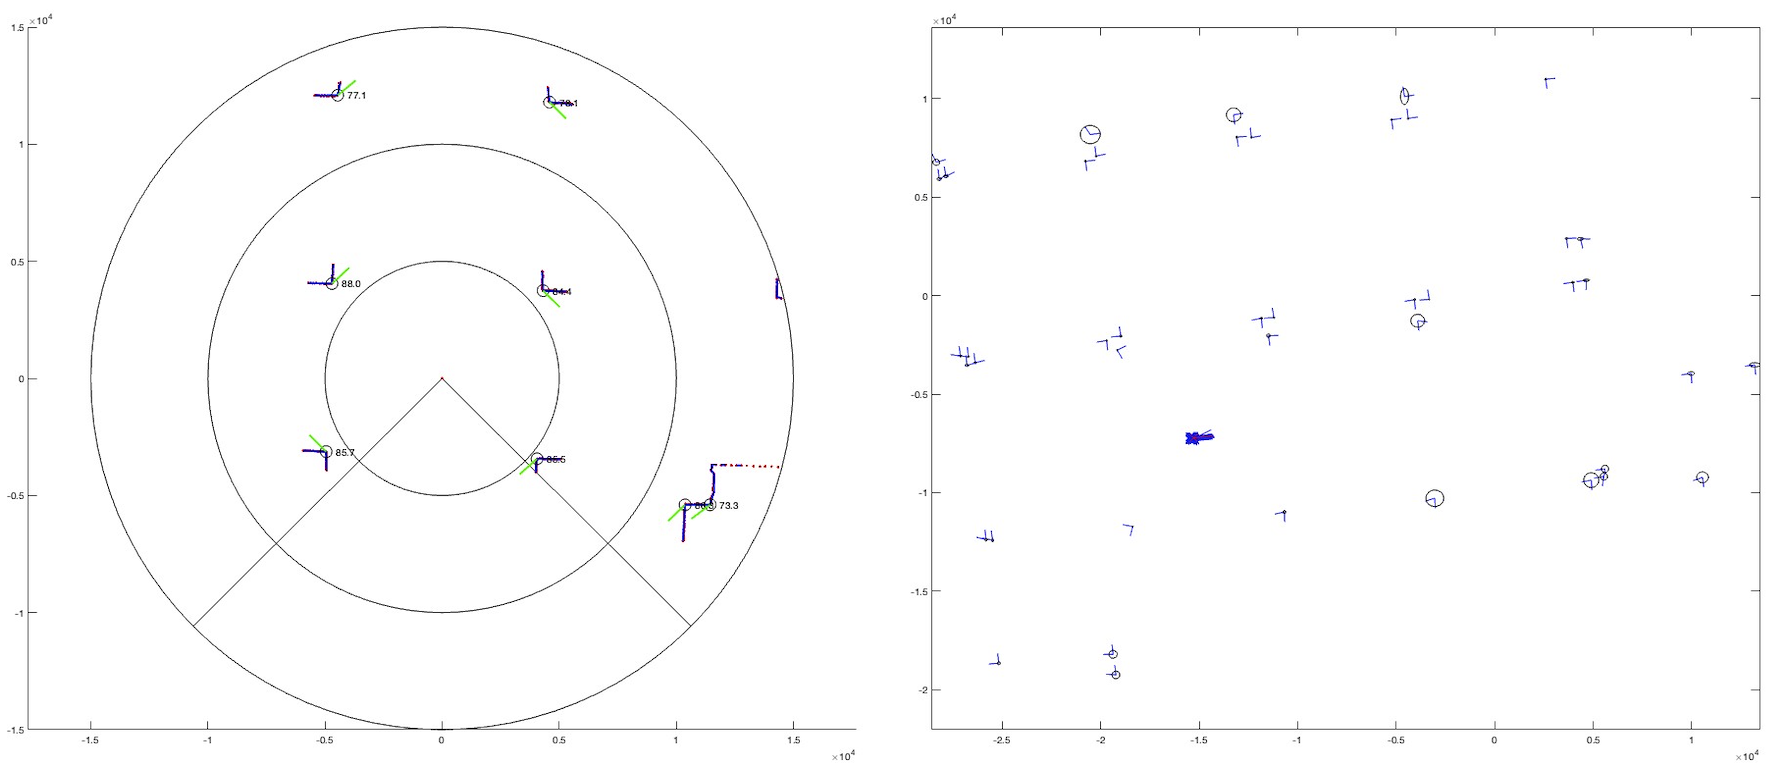
\includegraphics[width=1\linewidth, height=0.7\linewidth]{FastSLAM/SLAMsim.png}  
\caption{Simulation of Localization and Mapping using SLAM via Particle Filter}
\label{fig:SLAMSim}
\end{figure}